\chapter{Implementace}

V úvodu této kapitoly popíšeme koncepci programu, co kde
běží a jakým způsobem spolu komunikuje. Následně v sekci~\ref{analysis}
rozebereme zvolenou platformu a programovací jazyky,
další sekce budou pak věnovány popisu komponent, které jsme museli
naimplementovat pro funkci celého systému. Konkrétně jde o aplikaci pro
mobilní telefony s operačním systémem Android (v sekci~\ref{app}), vytvoření instance WA pro řízení
dialogu (s popisem získání nejběžnějších českých jmen pro trénink, \ref{wainit}) a komponenty
pro porovnání entit nalezených pomocí WA se seznamem kontaktů (\ref{matching}).

Jak jsme již uvedli, výsledkem je z uživatelského pohledu mobilní
aplikace. Většina vnitřních procesů však probíhá v cloudu, aplikace
je jen jakýmsi spojem a médiem pro komunikaci s uživatelem. Celý běh
je znázorněn na obrázku~\ref{img-flowchart}. Stisknutím tlačítka v
telefonu se
inicializuje session ve WA běžícím v cloudu IBM a spustí rozpoznávání řeči,
které běží na serverech Google. Po zahájení session ve WA jsou tam též
odeslána jména kontaktů uložených v telefonu. Jakmile je z hlasu rozpoznán
text, je vrácen zpět do aplikace a odtud odeslán jako zpráva do WA.
Ten rozhodne, zda je potřeba volat
porovnávací komponentu. Pokud ano, zavolá ji z jiné části IBM cloudu,
předá jí relevantní data a získá od ní odpověď. V každém případě
WA vygeneruje odpověď na zaslanou zprávu a odešle ji zpět do telefonu.
Tam je odpověď z WA zpracována (mj. je rozhodnuto, zda by měl být
zahájen hovor) a odeslána do syntetizátoru řeči na servery Google.
Odtud je hlas k přehrání vrácen zpět do aplikace, tam je přehrán
a následně je na základě dřívějšího rozhodnutí buď spuštěno znovu
rozpoznání hlasu, nebo je zahájen hovor a aplikace ukončena.


\begin{figure}[h]\label{img-flowchart}
    \centering
    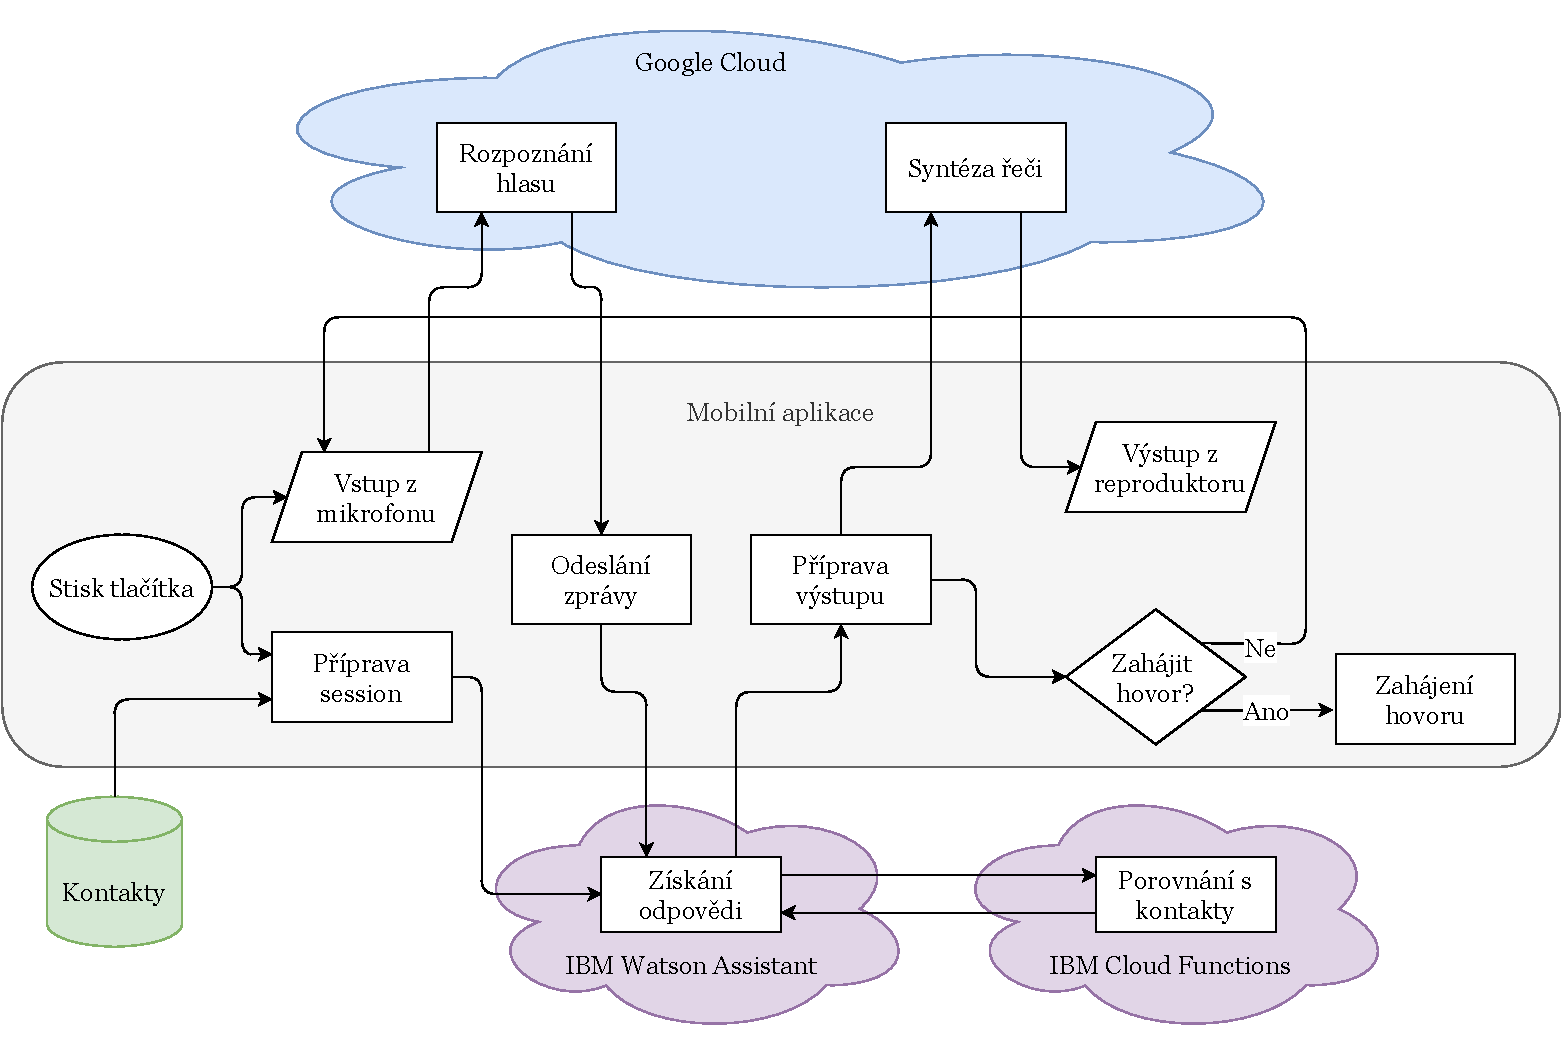
\includegraphics[width=0.98\textwidth]{../img/app-flowchart.pdf}
    \caption{Nákres fungování celého systému}
\end{figure}

\section{Platforma a programovací jazyky}\label{analysis}

\subsection{Platforma a jazyk mobilní aplikace}
Pro mobilní aplikace máme v dnešní době v zásadě dvě možnosti, iOS nebo Android.
Zvolili jsme Android, neboť je celkově otevřenější, autor telefon s tímto
operačním systémem vlastní a mají tedy alespoň uživatelské zkušenosti. IBM navíc
poskytuje vývojový balíček (\textit{SDK}) pro použití WA v programovacím
jazyku Java, který je použitelný i v Androidu.

Z hlediska programovacího jazyka padla volba na Kotlin. Existují různé frameworky
schopné zkompilovat pro Android program psaný téměř v libovolném programovacím
jazyce, ale většina nakonec musí používat nějakou další překladovou vrstvu.
Kotlin je jeden z jazyků, ve kterém lze psát nativní aplikace pro Android. Programy
v něm napsané lze totiž zkompilovat pro spuštění v \textit{JVM} (\textit{Java Virtual Machine}),
toto prostředí popisuje \citet{prof_tejinder_singh_hotspot_2014}.
Kotlin dokonce umožňuje interoperabilitu s Javou, což umožnilo
využití zmíněného SDK. Jeho výhoda oproti Javě je, že je celkově modernější,
psaní a čtení programů v něm je díky přehlednější syntaxi jednodušší a kratší,
navíc je doporučený samotnou firmou Google jakožto vedoucím vývoje operačního
systému Android \citep{android_blog}.
Další vlastností, na kterou při výběru nebyl brán tak velký
zřetel, ale nakonec se ukázala jako relativně zásadní, je podpora \textit{koprogramů}
(\textit{coroutines}), jejichž možnou implementaci ukazují \citet{theory_practice_coroutines}.

\subsection{Volba asistenta a jeho inicializace}
Frameworků pro tvorbu asistentů existuje na trhu mnoho, jen jeden však aktuálně oficiálně plně
podporuje český jazyk -- Watson Assistant od IBM. Proto zde volba jednoduše
padla právě na něj.

Inicializace WA lze provést v interaktivním prostředí v prohlížeči. Toto
prostředí je však v mnohém omezené. V našem případě jsme například potřebovali
vložit stovky entit pro trénování rozpoznání. Přenést je do WA přes prohlížeč
by bylo absurdně náročné, navíc složitě replikovatelné. Použili jsme proto opět
po SDK, pomocí kterého můžeme WA iniciovat relativně krátkým skriptem. Na volbě
konkrétního programovacího jazyka zde téměř nezáleželo (skript je krátký a běží
jen jednou pro inicializaci), zvolili jsme proto Python jakožto dobře čitelný
jazyk, se kterým máme mnoho zkušeností.

\subsection{Jazyk a prostředí běhu porovnávací komponenty}

Volba jazyka byla zde také jednoduchá, kolegové z MAMA AI totiž plánovali
komponentu také využít a požadovaným jazykem byl Python.

Při implementaci jsme potřebovali počítat podobnost řetězců. Algoritmus
pro tento výpočet je relativně komplikovaný a běžně používaný, nedávalo tedy
smysl programovat jej znovu. Využili jsme modul
\texttt{editdistance}\footnote{\url{https://pypi.org/project/editdistance/}},
protože je psaný v rychlejším jazyce C++ a má vhodnou licenci.

Dále bylo potřeba vyřešit, kde tato komponenta poběží. Nakonec jsme vybrali
službu IBM Cloud Functions. Původním nápadem bylo
zprovoznění webového serveru, který by vyřizoval požadavky na tuto komponentu.
To by však vyžadovalo další kód pro správu a především hardware, na kterém by
tento server běžel. Při hledání alternativ jsme dostali doporučení na
\textit{funkce poskytované jako služby} (\textit{function as a service, FaaS}),
které nabízí většina větších poskytovatelů cloudů. Jednoduše řečeno, na daný
server lze nahrát kód, který přijímá a vrací (obvykle) soubory formátu JSON a
běží jen ve chvíli, kdy dostane nějaký požadavek. Liší se tak od standardních
webových serverů, které musí \uv{poslouchat} neustále. Konkrétně byla vybrána
služba IBM Cloud Functions především proto, že lze spravovat ze stejného účtu jako
WA. Teoreticky může být výhoda využití stejného poskytovatele ještě v tom, že
servery budou na stejném místě a tedy výměna dat mezi nimi bude probíhat rychleji.

\section{Mobilní aplikace}\label{app}

Pro vytvoření aplikace jsme využili integrované vývojové prostředí
\textit{Android Studio}, které pro kompilaci využívá \textit{gradle}.
Původním záměrem bylo využít \textit{Visual Studio Code}
spolu s \textit{vývojovými kontejnery} za použití virtualizačního softwaru
\textit{Docker}, především díky přenositelnosti a relativní nenáročnosti
na výpočetní výkon. Ukázalo se však, že tato cesta není při vývoji aplikací
pro Android v jazyce Kotlin pod operačním systémem Windows úplně běžná a
naráží na mnoho komplikací. Od ruční inicializace projektu a vytvoření všech
potřebných souborů, přes design uživatelského
prostředí nutný čistě v textovém editoru a složitou správu závislostí,
až po problémy při kompilaci. Nakonec jsme tedy tuto cestu opustili a
musíme konstatovat, že především pro vývojáře začínající s Androidem
ji považujeme za silně nevhodnou.

Aplikace musela vyřešit několik věcí: získání oprávnění ke všem operacím,
získání kontaktů uživatele, vytvoření \textit{session} ve WA a odeslání
jmen kontaktů, spuštění rozpoznání hlasu, po dokončení jeho výsledek odeslat
jako zprávu do WA, po získání odpovědi spustit hlasový syntetizátor, po skončení
jeho projevu buď spustit rozpoznání hlasu a celý běh znovu, nebo zahájit
hovor. Všemi součástmi se budeme zabývat v následujících podsekcích, začneme
ale celkovou koncepcí a vzhledem.

\subsection{Celková koncepce a vzhled}

Jednotlivé komponenty (obvykle reprezentované jednou obrazovkou)
se v aplikacích
pro Android nazývají \textit{Activity}. Protože primárním způsobem interakce
s aplikací má být hlas, cílili jsme na jednoduché a sebevysvětlující grafické
rozhraní. Zvolili jsme tlačítko se symbolem mikrofonu na černém pozadí,
jak ukazuje obrázek~\ref{img-ui}. Tímto tlačítkem je zahájen dialog (v případě
dostatečných oprávnění, jejichž získání řešíme dále).

\begin{figure}[h]\label{img-ui}
    \centering
    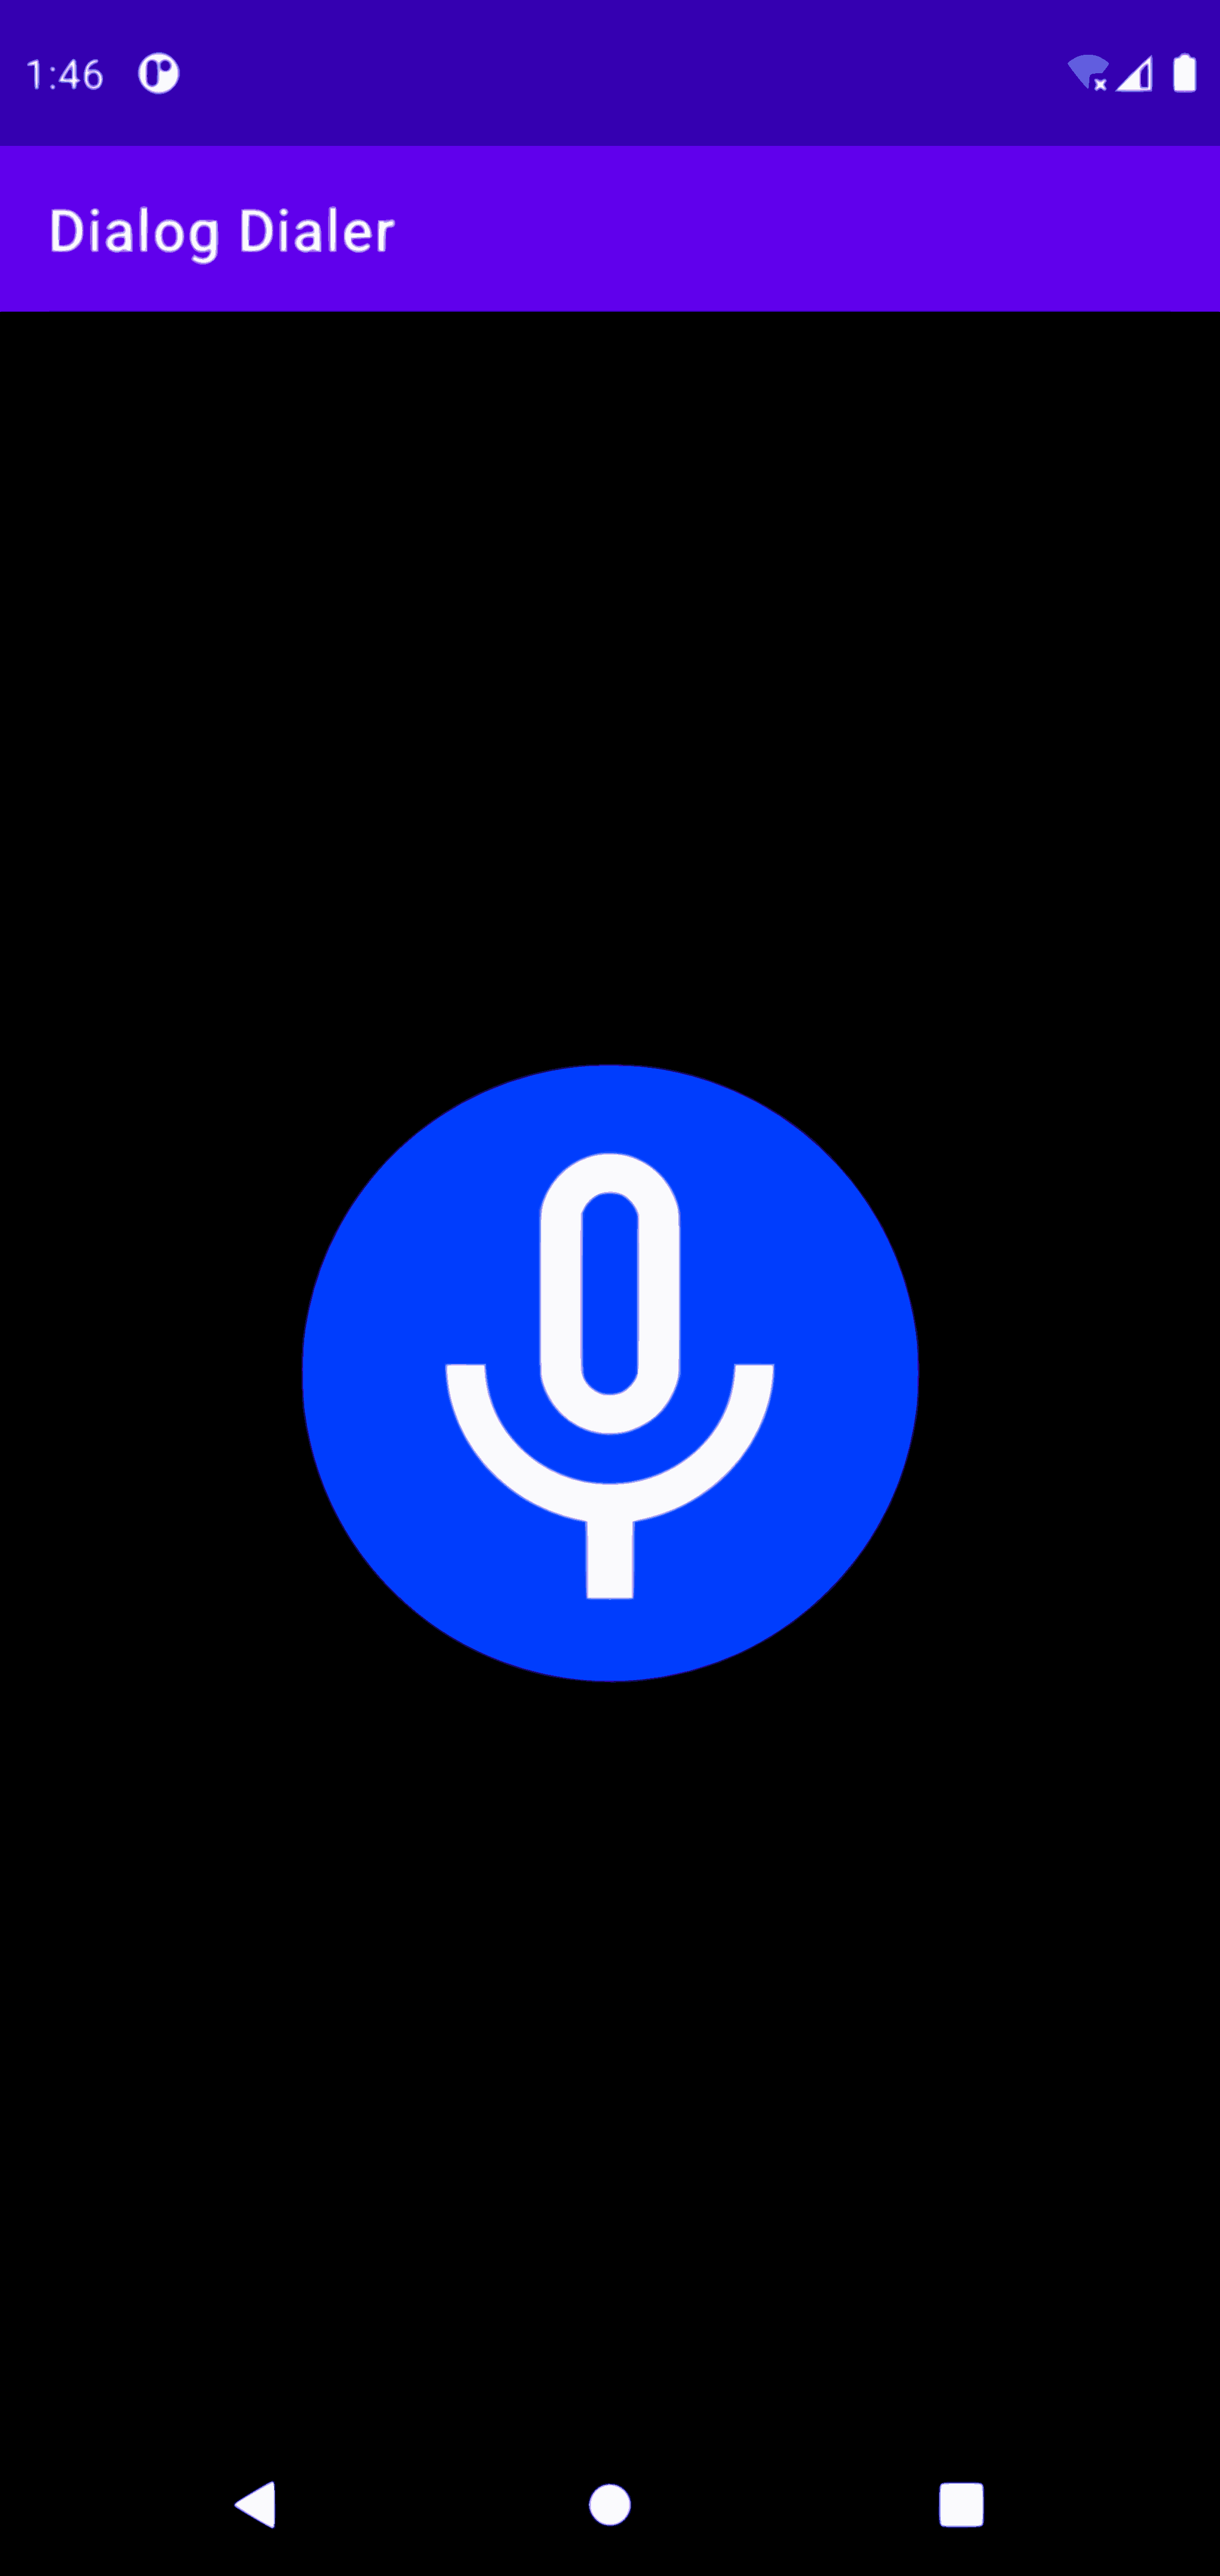
\includegraphics[width=0.3\textwidth]{../img/ui.pdf}
    \caption{Jednoduché uživatelské rozhraní}
\end{figure}

Protože nám stačí jedna obrazovka, je celý kód umístěn v jednom souboru
\texttt{MainActivity.kt}. Pro změnu grafického rozhraní z kódu je třeba
jejich propojení, které zajišťuje instance třídy \texttt{ActivityMainBinding}.
Toto je aktuálně oficiálně doporučený postup (na úkor dříve používaného
vyhledání pomocí \texttt{id}), ale vygenerování propojovací třídy musíme
povolit v souboru \texttt{build.gradle} na úrovni modulu.

Tato instance je využita při otevření aplikace pro \uv{nafouknutí} grafického
rozhraní a následně v kódu kdykoliv chceme k rozhraní přistupovat. To v našem
případě znamená nastavení reakce na stisk tlačítka, případně jeho deaktivace
či změna vzhledu pro indikaci probíhajících procesů.

\subsection{Získání oprávnění}

Pro svou správnou funkci potřebuje aplikace povolení nahrávat zvuk, číst
kontakty, vykonávat hovory a přistupovat k internetu. Všechna požadovaná
oprávnění musí být uvedena v souboru \texttt{AndroidManifest.xml}, první
tři jsou navíc oprávněními za času běhu, tedy o ně musíme explicitně
požádat. Oprávnění k přístupu k internetu není tak zásadní (především
protože neoperuje s uživatelovými daty), tedy je v Androidu automaticky
uděleno při instalaci aplikace.

Aktuálně oficiálně doporučeným postupem (který z toho důvodu využíváme), jak
řešit oprávnění, je nejprve o ně požádat, pokud uživatel odmítne a pokusí se
aplikaci znovu použít, zobrazit vysvětlení, k čemu jsou nutná a znovu o ně
požádat, a pokud znovu odmítne, již jen ukazovat upozornění o nedostupnosti.

Pro požádání o oprávnění potřebujeme spustit jinou aktivitu (pro získání
oprávnění existuje jedna vestavěná), vyčkat na její výsledek a na základě
něj rozhodnout o dalších krocích. K tomu využíváme opět aktuálně doporučenou
metodu \texttt{registerForActivityResult}. Pro zobrazení vysvětlení potřeby
oprávnění i upozornění o nedostupnosti využíváme třídu \texttt{AlertDialog}.

\subsection{Získání kontaktů}

Kontakty potřebujeme získat z úložiště telefonu, které se chová podobně jako
databáze. Proto dotaz na ně začneme na začátku inicializace celé služby WA
asynchronně jako koprogram. V rámci něj pak získáme jména a čísla kontaktů,
které uložíme do slovníku.

\subsection{Vytvoření session ve WA a odeslání jmen kontaktů}

Po začátku dotazu na kontakty vytvoříme instanci třídy \texttt{Assistant}
pro komunikaci s WA API, které předáme potřebné parametry a následně pošleme
požadavek pro zahájení session. V Androidu není možné posílat síťové požadavky
v hlavním vlákně (protože je potřeba udržovat ho volné pro UI), takže s výhodou
opět použijeme běh jako koprogram. Následně pomocí \texttt{await} zajistíme
kontrolu dokončení získávání kontaktů a předáme je jako \textit{kontext} do
WA session. Pokud se v průběhu něco nepovede, výjimku odchytíme a příště
se pokusíme provést celou inicializaci znovu.

Původní záměr byl odesílat kontakty do WA jako standardní zprávu, jenže
tam jsme brzy narazili na limit velikosti požadavku 2048 znaků. Delší
seznam kontaktů se do tohoto limitu nevejde, proto jsme nakonec využili
nastavení kontextu.

Důležité je ještě zmínit, že parametry pro komunikaci s WA jsou uloženy
zvlášť v souboru \texttt{credentials.xml}.

\subsection{Spuštění rozpoznávání hlasu}

Obdobně jako u získání
oprávnění potřebujeme spustit nějakou aktivitu a získat její výsledek, tedy
využijeme \texttt{registerForActivityResult}, tentokrát nejde o vestavěnou
aktivitu, ale můžeme využít parametr \texttt{Intent} (úmysl) při spuštění.
Protože ho potřebujeme používat často, vytvoříme ho jen jednou při otevření
aplikace a předáme mu potřebné parametry (český jazyk, jeden výsledek, atp.).
Když aktivita spuštěná s tímto úmyslem skončí, zkontrolujeme, že proběhla
úspěšně a pokračujeme k dalšímu kroku.

\subsection{Odeslání do WA a získání odpovědi}
Opět pomocí \texttt{await} vyčkáme nachystání WA. Pokud je vše připraveno,
pošleme v koprogramu (jedná se o síťový požadavek) text do WA a získáme odpověď.
Tuto odpověď ještě zpracujeme, pokud je na prvním řádku \texttt{[call]}, jedná
se o pokyn k hovoru, na druhém řádku najdeme jméno kontaktu a na třetím text k
přečtení. Pomocí jména kontaktu zjistíme jeho číslo, vytvoříme \texttt{Intent}
volání a nastavením proměnné \texttt{launchAgain} na \texttt{false} uložíme,
že dialog skončil. V opačném případě pošleme celou odpověď k přečtení.

\subsection{Spuštění hlasového syntetizátoru}

Převod textu na řeč budeme také potřebovat používat často, proto instanci
třídy \texttt{TextToSpeech} též vytvoříme při otevření programu. Nastavíme
ji na český jazyk a přepíšeme v ní funkci \texttt{onDone}, která je spuštěna,
když skončí přehrávání hlasu. Pokud dialog neskončil, spustíme celý běh
od rozpoznání hlasu zabalený ve funkci \texttt{launchPipeline} znovu. Pokud
skončil, jsme připraveni začít volat, vytočíme tedy číslo a ukončíme session ve
WA i celou aplikaci.

\section{Inicializace WA}\label{wainit}

Bohužel samotné vytvoření instance WA zatím není možné provést pomocí skriptů,
musíme ho tedy vytvořit ve webovém rozhraní. Odsud také získáme soubor
\texttt{ibm-credentials.env}, který budeme používat k autentizaci skriptů.

Když toto uděláme, jako první musíme vytvořit \textit{workspace}
(prostředí pro danou schopnost WA), což uděláme
jednoduchým požadavkem, který bude obsahovat parametry jako jméno nebo jazyk.
Zpět dostaneme odpověď, jejíž součástí bude \texttt{workspace\_id}, které budeme
dál potřebovat k manipulaci s prostředím. Pro úpravu tohoto prostředí
vždy budeme používat metodu \texttt{update\_workspace}, pomocí které můžeme
nahrát větší množství úprav naráz a nebudeme tak mít problémy s limitem na
počet požadavků.

\subsection{Úmysly a entity}

Jako první do něj přidáme detekci uživatelových úmyslů (intents), jejichž využití
jsme si představili v podsekci~\ref{nlu}. Zásadní je úmysl
\texttt{dial}, pomocí kterého detekujeme, že uživatel chce někomu volat. Pro
každý úmysl přidáme několik vzorových vět, na základě kterých by ho měl WA
rozpoznat. Ty jsou interně použity pro trénink umělé modelu stojícího za WA.
Obdobně vytvoříme zbývající úmysly \texttt{greet} a \texttt{bye}, aby náš
asistent uměl slušně pozdravit.

Jediné entity, které potřebujeme rozeznávat, jsou jména lidí, případně příjmení.
Do WA je k tréninku dostaneme obdobně jako úmysly. Uvažovali jsme, jak ale tato
data získat. Nakonec jsme využili data četnosti jmen a příjmení MVČR z roku 2017.
Sice již přímo na stránkách MVČR nejsou dostupná, ale ve ve webových archivech
existují. Tato data byla uložena ve formátu \texttt{xls} ve více listech, pro
počítačové zpracování ne moc ideálním. Pomocí knihovny \texttt{pandas} jsme je
tedy převedli do formátu \texttt{csv}, kde byla i výrazně menší. Následně jsme
vybrali všechna jména i příjmení, která v Česku k roku 2017 nosilo alespoň
200 (TODO check hranice) lidí a ta jsme nahráli do WA.

\subsection{Stavba dialogu}

Nejkomplikovanější částí bylo samotné sestavení průběhu dialogu s odesláním
dat do porovnávací komponenty. (TODO možná přesunout do popisu WA?) WA využívá
\textit{stromovou} reprezentaci dialogu,
kde sekvenčně kontrolujeme splnění podmínky (detekci úmyslu nebo entity) v
jednotlivých sourozencích. Jakmile v jednom najdeme podmínku splněnou, vybereme
odpověď z něj a pokud nějaké má, zanoříme se do jeho synů. Ve webovém rozhraní je
stavba dialogového stromu relativně přímočará, ale v některých místech omezená,
proto jsme i zde použili skript.

Vytváření dialogového stromu ve WA pomocí Python SDK je poněkud komplikovanější
než přes webové rozhraní. Například pokud chceme, aby vrchol vyžadoval zaplnění
určitého slotu a rozpoznanou hodnotu v něm ukládal do kontextu, musíme pro
každou tuto operaci vyrobit jeden podvrchol, zatímco v rozhraní bychom jen
vyplnili dvě pole.

Celkově je povrchová koncepce stromu relativně jednoduchá. Máme sourozenecké
vrcholy pro detekci uživatelových úmyslů pozdravit, zavolat a rozloučit se, navíc
dva speciální. Ty zajistí, že na začátku dialogu asistent nic neříká, a že
pokud není detekován žádný úmysl, asistent se na něj zeptá. Jediným vrcholem
s potomky je vrchol detekující úmysl volat, který ještě kontroluje zaplnění slotu
pro jméno (případně se na něj doptá). Nepřišli jsme na to, jak přímo z něj
uložit vstup a rozpoznané entity do kontextu, proto jeho syn dělá právě to. Ten
má dalšího syna, který relevantní kontext (vstup, rozpoznané entity a kontakty)
odešle do \textit{webhooku} (v zásadě webová adresa očekávající vstup a vracející
výstup, oboje ve formátu JSON), kde běží porovnávací komponenta. Získá tak její
výstup a na základě něj generuje odpověď -- pokud dostal zpět jedno jméno,
vyzve k zahájení hovoru; pokud více, vyzve k vybrání (a nastaví je do kontextu,
aby příště bylo porovnáváno jen s nimi); pokud žádné, oznámí že nic neodpovídá.
Poté se vrátí do uzlu připravujícího údaje, aby mohlo být provedeno případné
upřesnění.

TODO možná obrázek stromu?

\section{Porovnávací komponenta}\label{matching}

Tuto komponentu jsme implementovali pro obecné použití v dialogových systémech
v rámci knihovny \texttt{mConversation} MAMA AI, součástí jsou desítky testů
využívající frameworku \texttt{pytest}. Za účelem využití v aplikaci jsme komponentu
drobně upravili pro kontext vybírání z telefonního seznamu. Proto zde první popíšeme
obecnou část cílů a implementace, a pak konkrétní provedené úpravy.

Vstupem komponenty jsou entity rozpoznané pomocí WA, původní textový vstup do něj
a určitý (obvykle vázaný na uživatele) seznam entit. Cílem je vybrat entitu ze seznamu,
která nejvíce odpovídá vstupu do WA. V úvahu přitom nejsou brány jen entity, které
WA rozpoznal, ale i originální vstup. Pokud tak například uživatel zmíní běžné jméno a
neběžné příjmení, a WA rozpozná jako entitu jen jméno, komponenta dokáže najít a využít
i příjmení, takže pravděpodobně vrátí pouze jeden kontakt. Kdyby ho v úvahu nevzala,
vrátí všechny kontakty odpovídající jménu (s jinými příjmeními).

Součástí je i příprava pro určité rozšíření využívající strojového učení -- každý
uživatel by měl mít uložený svůj model, který se naučí jeho preference a bude se
průběžně zlepšovat využitím zpětné vazby. To je ale zatím jen koncept.

\subsection{Předzpracování}

K seznamu kontaktů si vytvoříme slovník,
který jako klíče bude mít všechny části kontaktů a jako hodnoty indexy do původního
seznamu. Tedy například pokud máme v seznamu na prvním místě kontakt \uv{Jan Novák},
ve slovníku budou \uv{Jan} i \uv{Novák} odkazovat na index 1.

Podobně předzpracujeme i rozpoznané entity, pro rychlý přístup k informacím o nich
využijeme opět slovník. Navíc pokud WA rozpoznal dvě entity v navazujících úsecích vstupu,
spojíme je dohromady, pravděpodobně se totiž jedná právě třeba o jméno a příjmení.
Pokud WA v nějakém segmentu rozpoznal více entit a má dojít k tomuto spojování, spojíme
je ve všech různých kombinacích (nějaká rozpoznaná je pravděpodobně chybná).

\subsection{Vlastní porovnávání}

Kdykoliv budeme porovnávat nějaké řetězce, využijeme tzv. \textit{fuzzy matching}.
To znamená, že řetězce nebudeme porovnávat přímo, ale pomocí Levenshteinovy vzdálenosti
zmíněné v podsekci~\ref{nlu}. Tím umožníme přiřazení ke kontaktu i při nepřesné shodě,
ať už není shoda úplná kvůli jinému tvaru slova (skloňování), chybě v rozpoznání
hlasu, nebo chybě rozpoznání entity ve WA. Jako odpovídající pak označíme kontakty,
jejichž vzdálenost je menší nebo rovna nějakému limitu. Jako limit maximálního počtu
úprav jsme zvolili 3. Je dost vysoký na to, aby ještě přijal například slovo s příponou
\uv{-ovi}, na druhou stranu vyšší limity způsobují přiřazení i řetězců neodpovídajících,
zvláště u krátkých slov (i s tímto limitem můžeme ke slovu délky 3 přiřadit libovolné jiné
stejné délky 3, protože nám stačí vyměnit 3 znaky). Pokud celé entitě nic neodpovídá,
zkusíme ji rozdělit podle mezer a porovnat jednotlivé části.

Každému přiřazenému kontaktu pak ještě určíme \textit{jistotu} (\textit{confidence}),
s jakou jsme ho přiřadili. Tu jsme se rozhodli počítat jako
\[ \text{confidence} = 0,5 + \frac{0,5 \cdot (\text{edit\_limit} - \text{distance})}{\text{edit\_limit}} ,\]
protože pak řetězce odpovídající přesně dostávají plnou jistotu, zatímco řetězce na
hraně limitu jistotu poloviční.

Poté ještě vezmeme v úvahu originální vstup, kdyby WA něco nerozpoznal. U každého
úseku vstupu, který byl přiřazen nějakému kontaktu, se díváme na předchozí a následující
slovo, zda neodpovídá stejnému kontaktu. Porovnání uděláme stejně jako v první fázi.
Pokud najdeme slovo, kde tomu tak je, rozšíříme úsek přiřazený k tomuto kontaktu.

Dále z rozpoznání vyřadíme kontakty, které odpovídají jen podúseku jiného
přiřazeného kontaktu. To se může stát právě pokud jednomu úseku odpovídalo více
kontaktů, ale jen jeden z nich jsme rozšířili kontrolou okolních slov. Vyřadíme také
všechny přiřazené kontakty, jimž jsme udělili jistotu menší než 0,5.

Nakonec vytvoříme finální výstup sestávající ze slovníku indexů přiřazených kontaktů
do původního seznamu, kde jako hodnoty budou opět slovníky s názvem kontaktu (jen pro
jednoduchost) a s jistotou přiřazení.

\subsection{Provedené úpravy a integrace}

Původně komponenta brala jako vstup seznam kontaktů ve formátu, v jakém jsou uložené
entity ve WA. Pro toto použití ho však dostáváme na vstupu ve formátu JSON, proto
jsme seznam uložili do slovníku pod klíč \texttt{\_\_contacts\_\_}.

Druhou změnu jsme provedli na výstupu, protože potřebujeme, aby komponenta provedla
celé rozhodnutí a vrátila něco, co může WA dobře zpracovat. Proto pokud u nějakého
přiřazeného kontaktu vyjde jistota o více než 0,1 vyšší než u jiných, odpovídá asi
výrazně více než jiné a vrátíme pouze
ten, jinak vrátíme seznam přiřazených (bez indexů a jistot, jen názvy).

Jak jsme již zmínili, celé porovnávání běží v IBM Cloud Functions. Tam je však možné
importovat jen jeden soubor s hlavní metodou \texttt{main}, která se vykoná při
příchodu požadavku a vrátí výsledek. Proto jsme celý relevantní kód umístili do
jednoho souboru. Nakonec jsme však zjistili, že musíme přibalit ještě využívaný
modul \texttt{editdistance}. Zde jsme jako nejjednodušší variantu získání importovatelného souboru
zvolili vytvoření \textit{virtualenv} s instalovanými potřebnými moduly,
který jsme zabalili spolu s vlastním kódem v souboru s názvem \texttt{\_\_main\_\_.py}
(toto jméno je povinné) do jednoho ZIP archivu a ten jsme úspěšně nahráli.